\subsection{数据处理与EDA}

\subsubsection{数据预处理}

本文的来自题目附件 Telco\_customer\_churn.xlsx, 包含了$7043$条客户数据记录，共33个字段，
涵盖客户人口统计学信息、账户信息、服务订阅信息和流失标签。

本文首先利用pandas将 Telco\_customer\_churn.xlsx文件转换为csv文件，以便后续对数据进行处理。
接着本文读取了数据文件的基本信息，对数据进行了清洗，剔除了 CustomerID、Count、Country 三列。
我们剔除这三列的依据是第一，CustomerID 作为唯一标识，与客户流失情况无关，无泛化预测能力；
第二，Count 恒为1，方差为0，对区分客户无贡献；第三，Country，全部为 United States，无差异性，对
模型无额外信息量。

其次，在完成数据清洗工作之后，本文发现 \texttt{Total Charges}
为字符串类型，不便于后续对数值数据的处理。
于是，\texttt{Total Charges} 列的数据经 \texttt{pd.to\_numeric}
转换后确认 11 条 \texttt{NaN} 记录。通过追溯发现这 11 条记录的
\texttt{Tenure Months} 均为 0（新客户尚未产生消费）；因此填充为 0，
符合正常的业务逻辑。处理后全部 7043 行无缺失值。

最后，本文为了更加方便地识别各列数据的含义，对部分关键数据的列名，进行了中英翻译，提供列名对照表如表 \ref{tab:variable_mapping} 所示。
后续分析将统一使用中文名称。

\begin{table}[H]
    \centering
    \caption{关键变量名称对照表}
    \label{tab:variable_mapping}
    \small
    \begin{tabular}{clll}
        \toprule
        {\heiti 变量类别} & {\heiti 中文名称}
        & {\heiti 原始列名} & {\heiti 说明} \\
        \midrule
        目标变量 & 是否流失 & Churn Value
        & 1=流失, 0=未流失 \\
        \addlinespace
        \multicolumn{4}{l}{\heiti \small （一）时长与费用特征} \\
        数值 & 在网时长 & Tenure Months & 单位：月 \\
        数值 & 月消费金额 & Monthly Charges & 单位：美元 \\
        数值 & 总消费金额 & Total Charges & 单位：美元 \\
        数值 & 客户生命周期价值 & CLTV & Customer Lifetime Value \\
        \addlinespace
        \multicolumn{4}{l}{\heiti \small （二）合同与支付特征} \\
        分类 & 合同类型 & Contract & 月付/一年/两年 \\
        分类 & 支付方式 & Payment Method & 共 4 种 \\
        二分类 & 是否无纸化账单 & Paperless Billing & Yes / No \\
        \addlinespace
        \multicolumn{4}{l}{\heiti \small （三）服务订阅特征} \\
        多分类 & 互联网服务类型 & Internet Service & DSL/Fiber optic/No \\
        二分类 & 在线安全服务 & Online Security & Yes/No/No internet \\
        二分类 & 技术支持服务 & Tech Support & Yes/No/No internet \\
        \addlinespace
        \multicolumn{4}{l}{\heiti \small （四）人口与家庭特征} \\
        二分类 & 是否老年人 & Senior Citizen & Yes / No \\
        二分类 & 是否有配偶 & Partner & Yes / No \\
        二分类 & 是否有家属 & Dependents & Yes / No \\
        \addlinespace
        \multicolumn{4}{l}{\heiti \small （五）其他说明} \\
        文本 & 客户编号 & CustomerID & 无预测价值，已剔除 \\
        数值 & 纬度 & Latitude & 与流失相关系数<0.01 \\
        数值 & 经度 & Longitude & 与流失相关系数<0.01 \\
        \bottomrule
    \end{tabular}
\end{table}

\subsubsection{流失客户特征探索}

\subsubsection*{整体流失率}

本文首先对数据的整体客户流失情况，进行了分析以了解各类别的分布特征。以 Churn Value 为分类依据，统计得到客户流失$1869$人，
未流失客户$5174$人，总客户$7043$人，整体流失率为$26.54\%$，如图 \ref{fig:churn_rate} 所示

\begin{figure}[H]
    \centering
    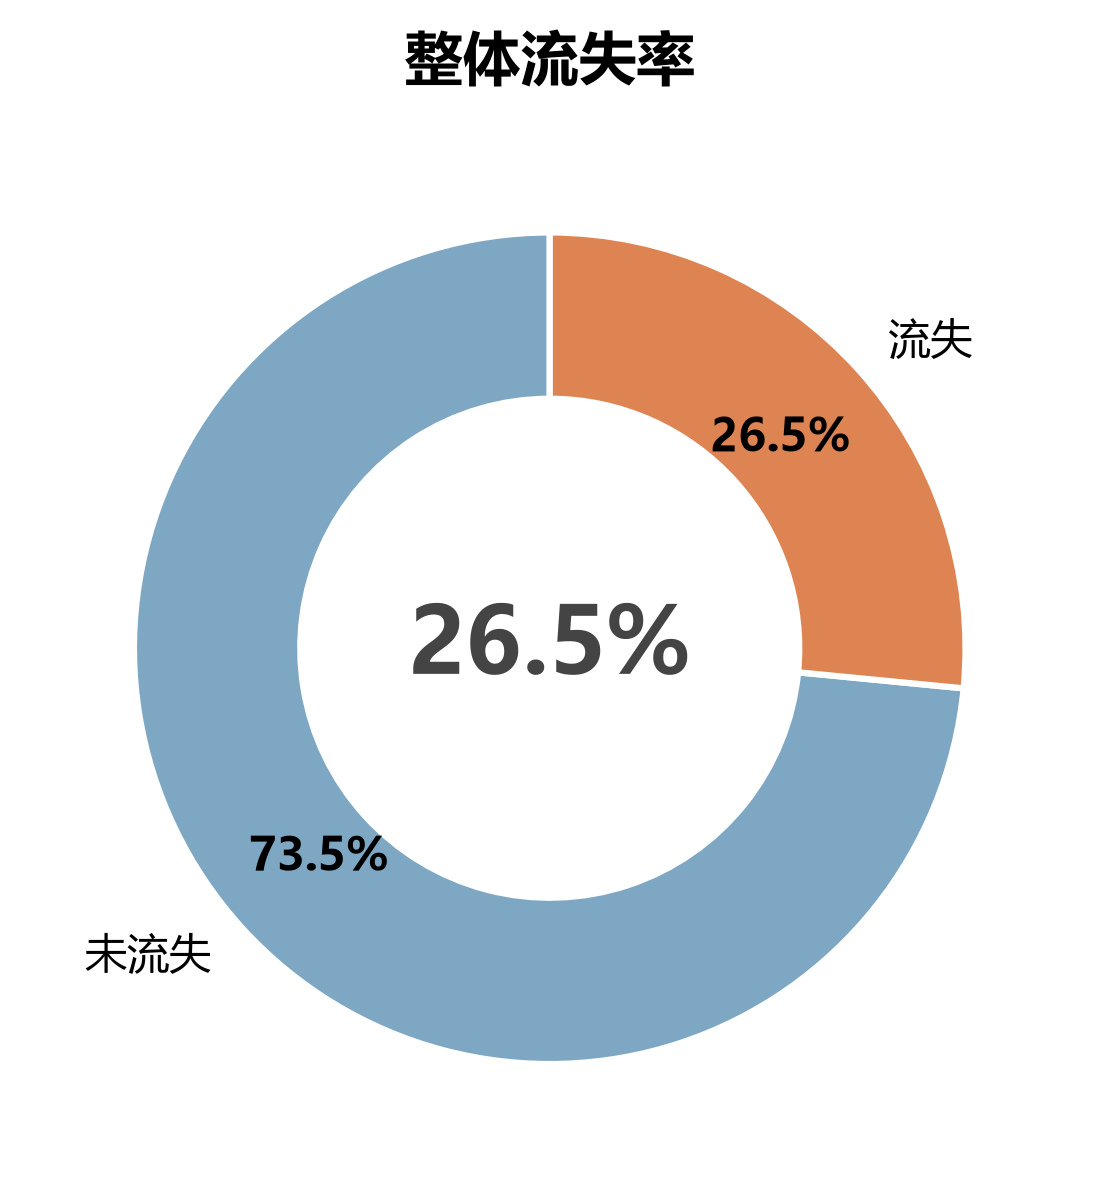
\includegraphics[width=0.5\textwidth]{figures/整体流失率.png}
    \caption{整体流失率环形图}
    \label{fig:churn_rate}
\end{figure}

从分布比例来看，流失与未流失两类样本的比例约为 1:2.8，呈现一定程度的类别不均衡。这一比例虽然不属严重失衡（如 1:10 以上），
但已足以对常规分类模型的训练过程产生影响——模型倾向于将多数类（未流失）识别得更好以降低整体损失，而牺牲对少数类（流失）的识别能力。
例如，一个将所有样本都预测为"未流失"的简单模型也能获得 $73.46\%$ 的准确率，但这显然不能反映模型在实际业务中的价值。

针对上述问题，本文在后续建模中采取以下应对措施：一是在评价指标上，不采用对不平衡数据敏感的准确率（Accuracy），
而采用 AUC（ROC 曲线下面积）和 F1-score 作为主要评价指标；二是在模型训练上，对逻辑回归设置 class\_weight='balanced' 参数，
使模型根据类别频率自动调整权重，强化对流失客户的关注。

\subsubsection*{整体流失率}

其次，为考察流失客户与未流失客户在数值特征上的分布差异，本文选取了选取在网时长（Tenure Months）、
月消费金额（Monthly Charges）和总消费金额（Total Charges）三个具有明确的业务含义的核心数值特征，
分别绘制分组直方图与箱线图进行对比，如图 \ref{fig:num_features} 所示。

\begin{figure}[H]
    \centering
    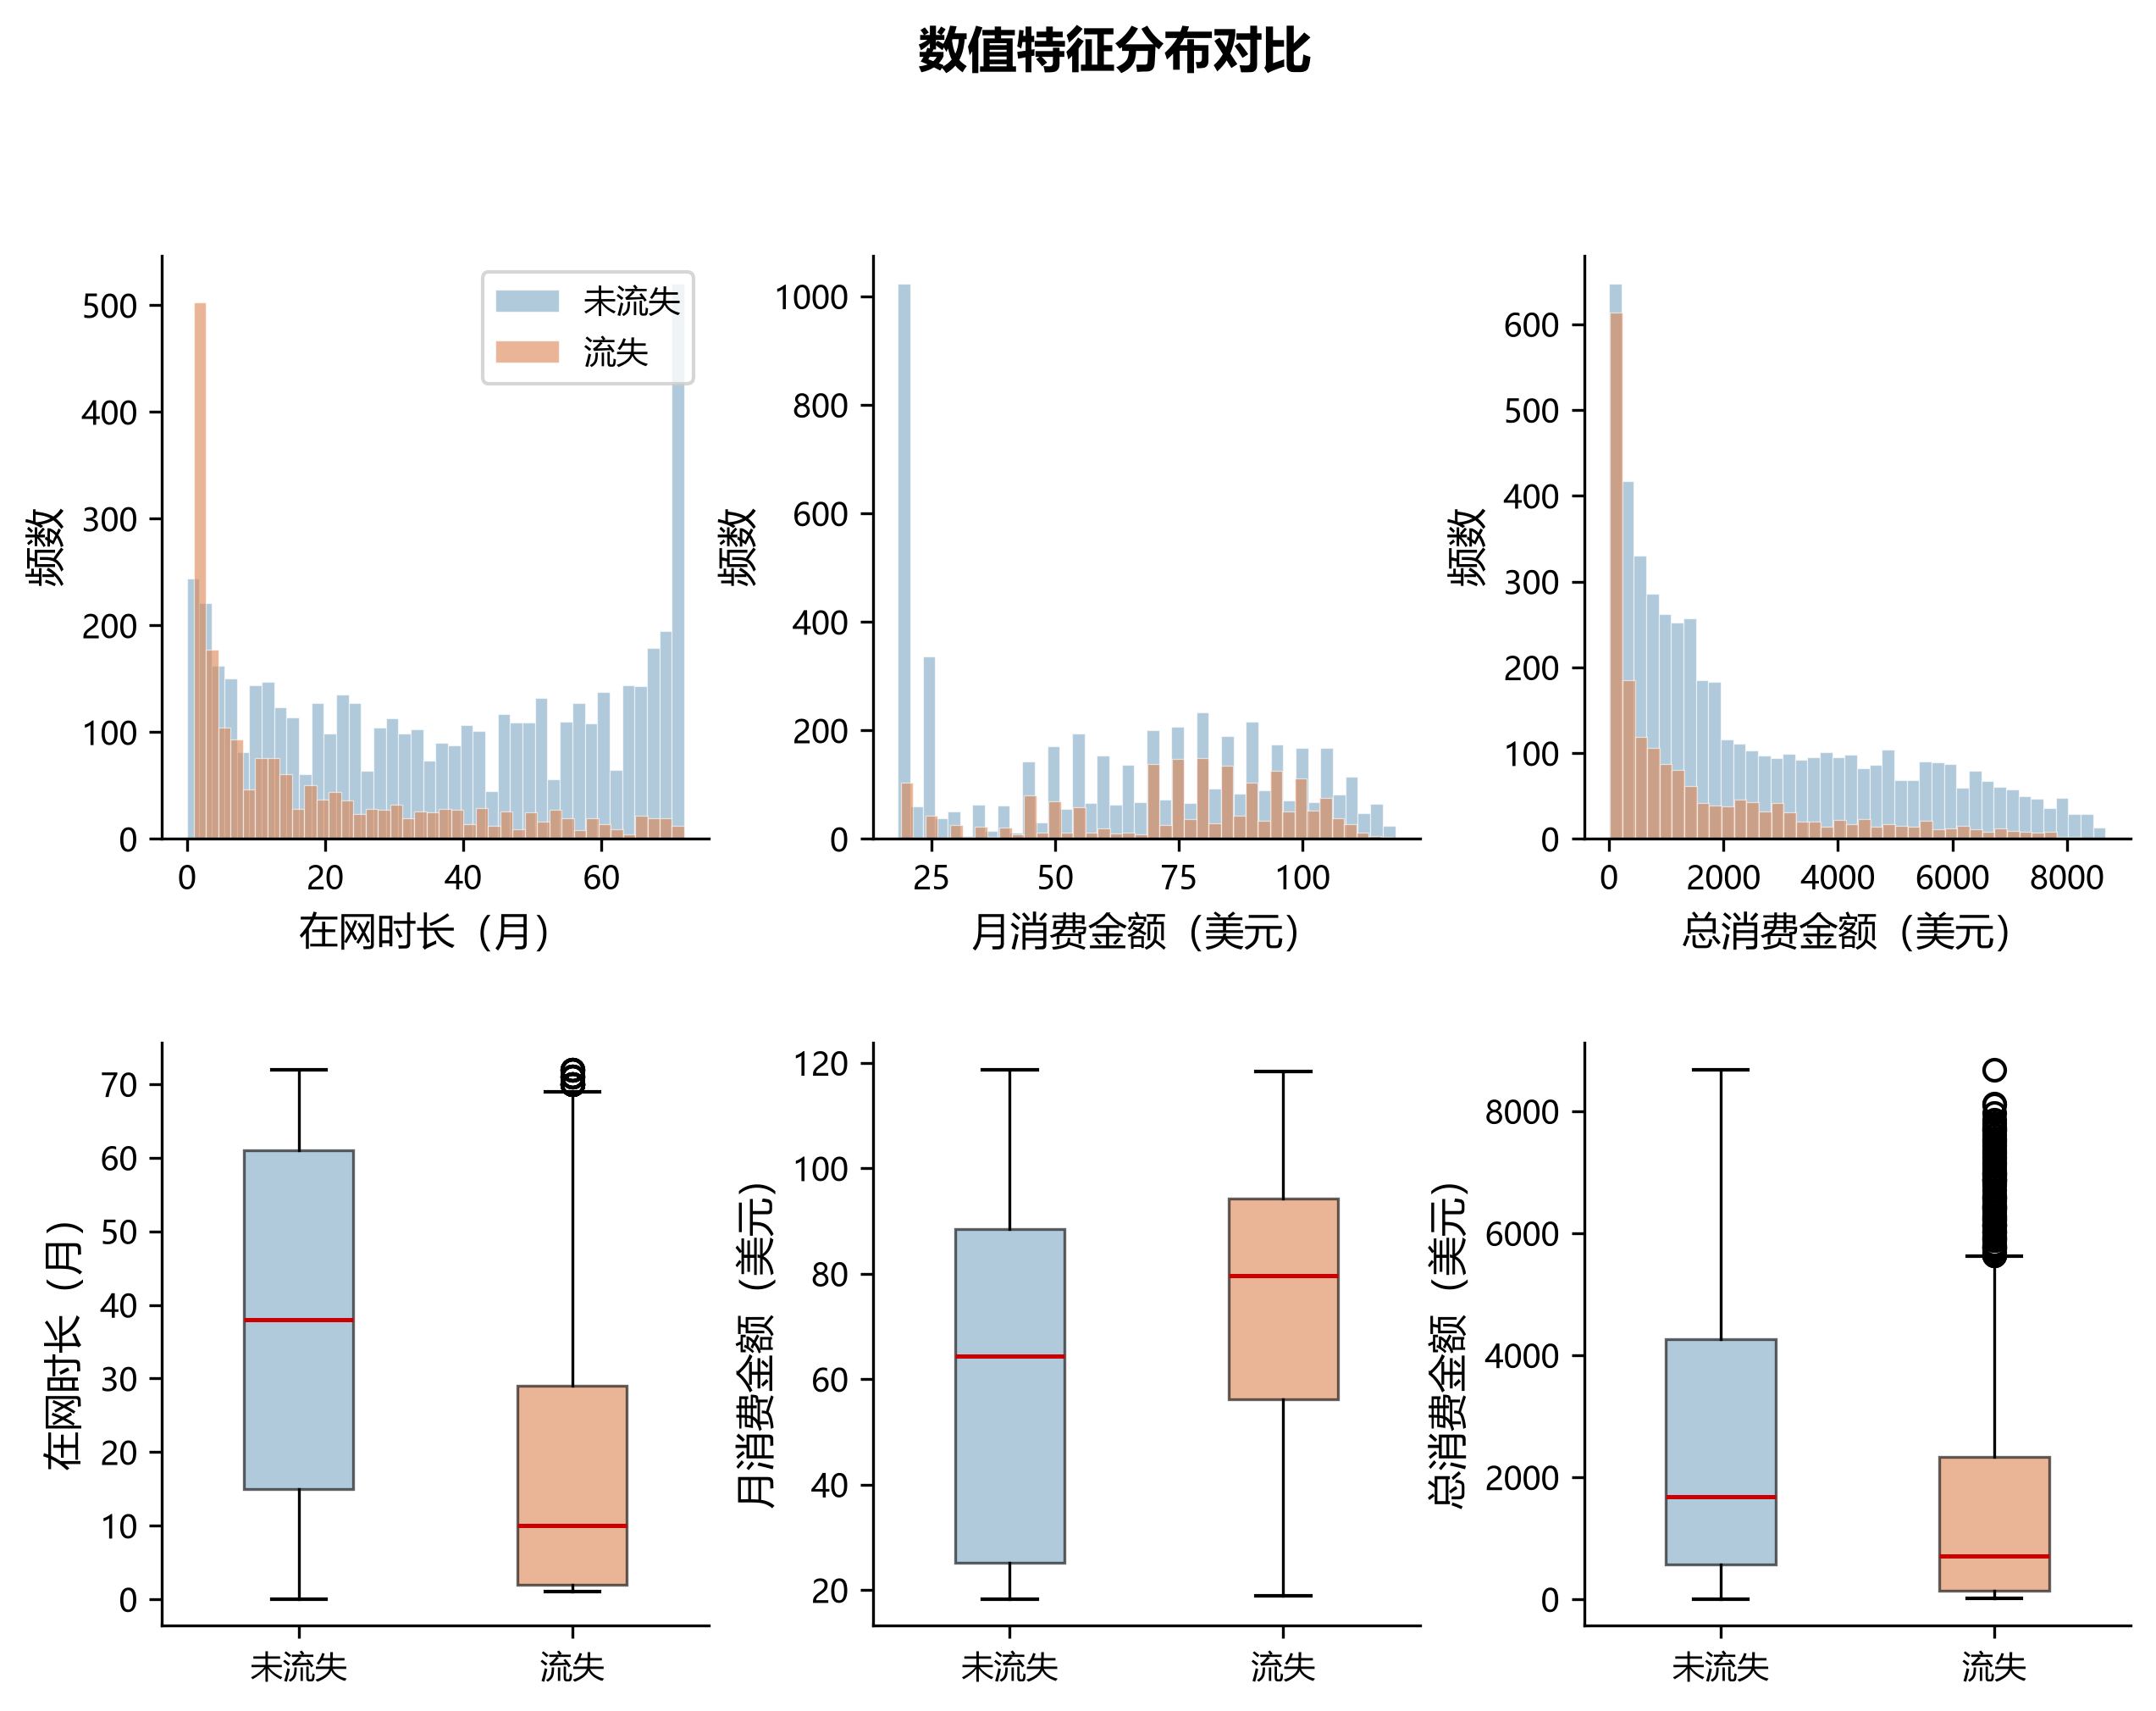
\includegraphics[width=0.85\textwidth]{figures/数值特征分布对比.png}
    \caption{数值特征分布对比图}
    \label{fig:num_features}
\end{figure}

本文通过对这三个特征的直方图和箱线图的分析，得到了这些特征与客户流失情况存在的关联如下：

\textbf{在网时长：}流失客户的分布高度集中于 0-10 个月的低在网时长区间，而未流失客户的分布较为均匀，
覆盖 0-72 个月的全区间。箱线图显示两组中位数差距显著，说明在网时长是区分能力最强的数值特征——新客户是流失的高风险群体。

\textbf{月消费金额：}流失客户的月消费整体偏高，在 70-110 美元的高费区间聚集密度明显大于未流失客户。
高消费客户对价格更为敏感，流失意愿相对更强。

\textbf{总消费金额：}流失客户的总消费明显偏低且呈左偏分布，但该差异主要源于在网时长短导致的消费积累不足，
属于在网时长的间接效应，其独立区分能力有限。

综合以上分析，在网时长是区分流失与未流失最有效的数值特征。

\subsubsection*{分类特征流失率对比}

然后本文为考察分类变量各取值水平下的流失风险差异，选取合同类型、互联网服务类型、支付方式、是否老年人、是否有配偶、
是否有家属、是否开通电话服务、是否无纸化账单共 8 个分类特征，分别统计各组流失率并绘制柱状图，如图 \ref{fig:cat_features} 所示。

\begin{figure}[H]
    \centering
    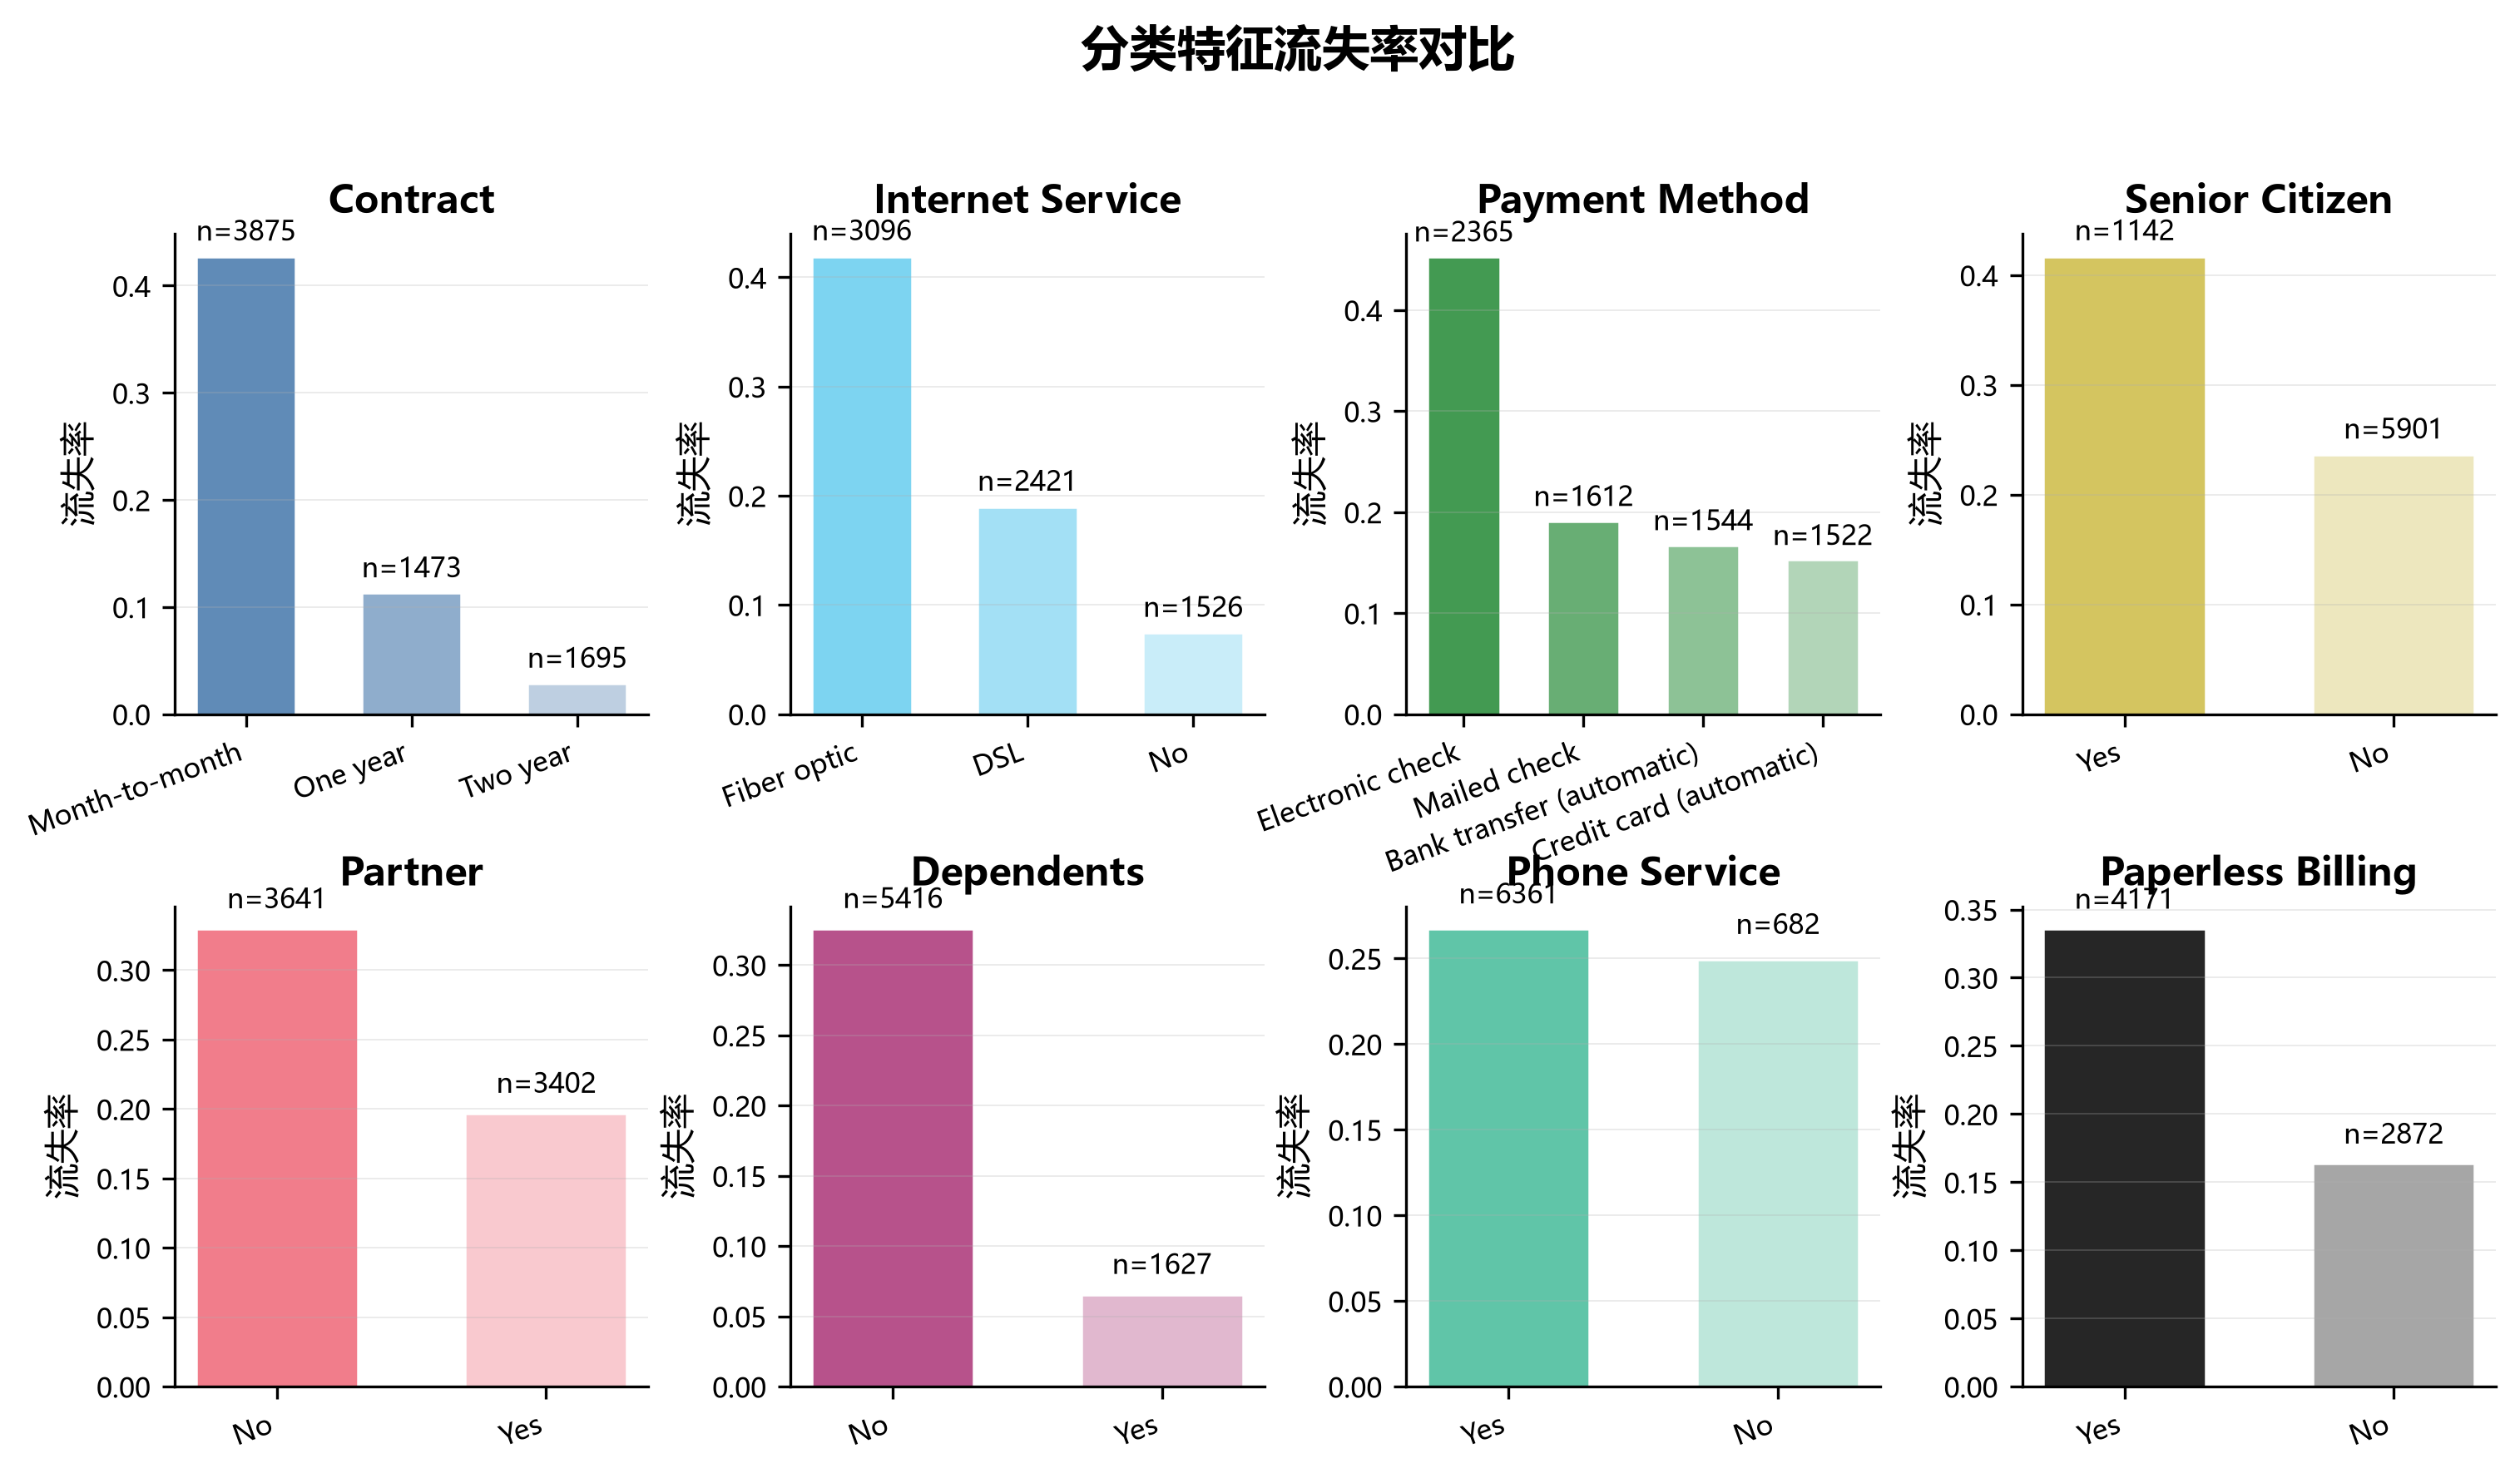
\includegraphics[width=0.85\textwidth]{figures/分类特征流失率对比.png}
    \caption{分类特征流失率对比图}
    \label{fig:cat_features}
\end{figure}

本文结合图中反映的各个特征不同组别类型的流失率和流失人数，发现了各个特征的客户流失的特点如下：

\textbf{合同类型（Contract）：}月付合同的流失率超过 40\%，而一年合同约为 10\%、两年合同约为 3\%。合同期限的差异根本性地改变了客户流失的
转换成本——月付客户可以随时解约，而年付和两年合同的客户通常承担了提前解约的违约金或已享受合约折扣，转换运营商的意愿显著降低。

\textbf{互联网服务类型（Internet Service）：}光纤客户的流失率显著高于 DSL 客户和无互联网客户，可能与光纤服务的
高月费有关——高消费群体对服务性价比的要求也更高。

\textbf{支付方式（Payment Method）：}电子支票客户的流失率约为 45\%，而银行自动转账、
信用卡自动支付和邮寄支票三种方式的流失率均在 15\%-20\% 之间，表明支付方式与客户属性之间存在一定的关联性。

此外，有配偶或有家属的客户流失率低于独身客户（家庭绑定提高了离网成本），无纸化账单客户流失率高于纸质账单客户（无纸化账单客户更习惯线上操作，
对运营商的服务切换成本感知较低，更容易比价和更换服务商），而是否老年人和是否开通电话服务对流失率的影响相对较小。

\subsubsection*{相关性热力图}

最后，本文采用 Pearson 相关系数衡量各数值特征与流失之间的线性关联强度，
相关系数的取值范围为 $[-1, 1]$，绝对值越接近 1 表示线性相关越强。
本文据此计算了数值变量的相关系数矩阵，并以热力图形式呈现，
如图 \ref{fig:corr} 所示。

\begin{figure}[H]
    \centering
    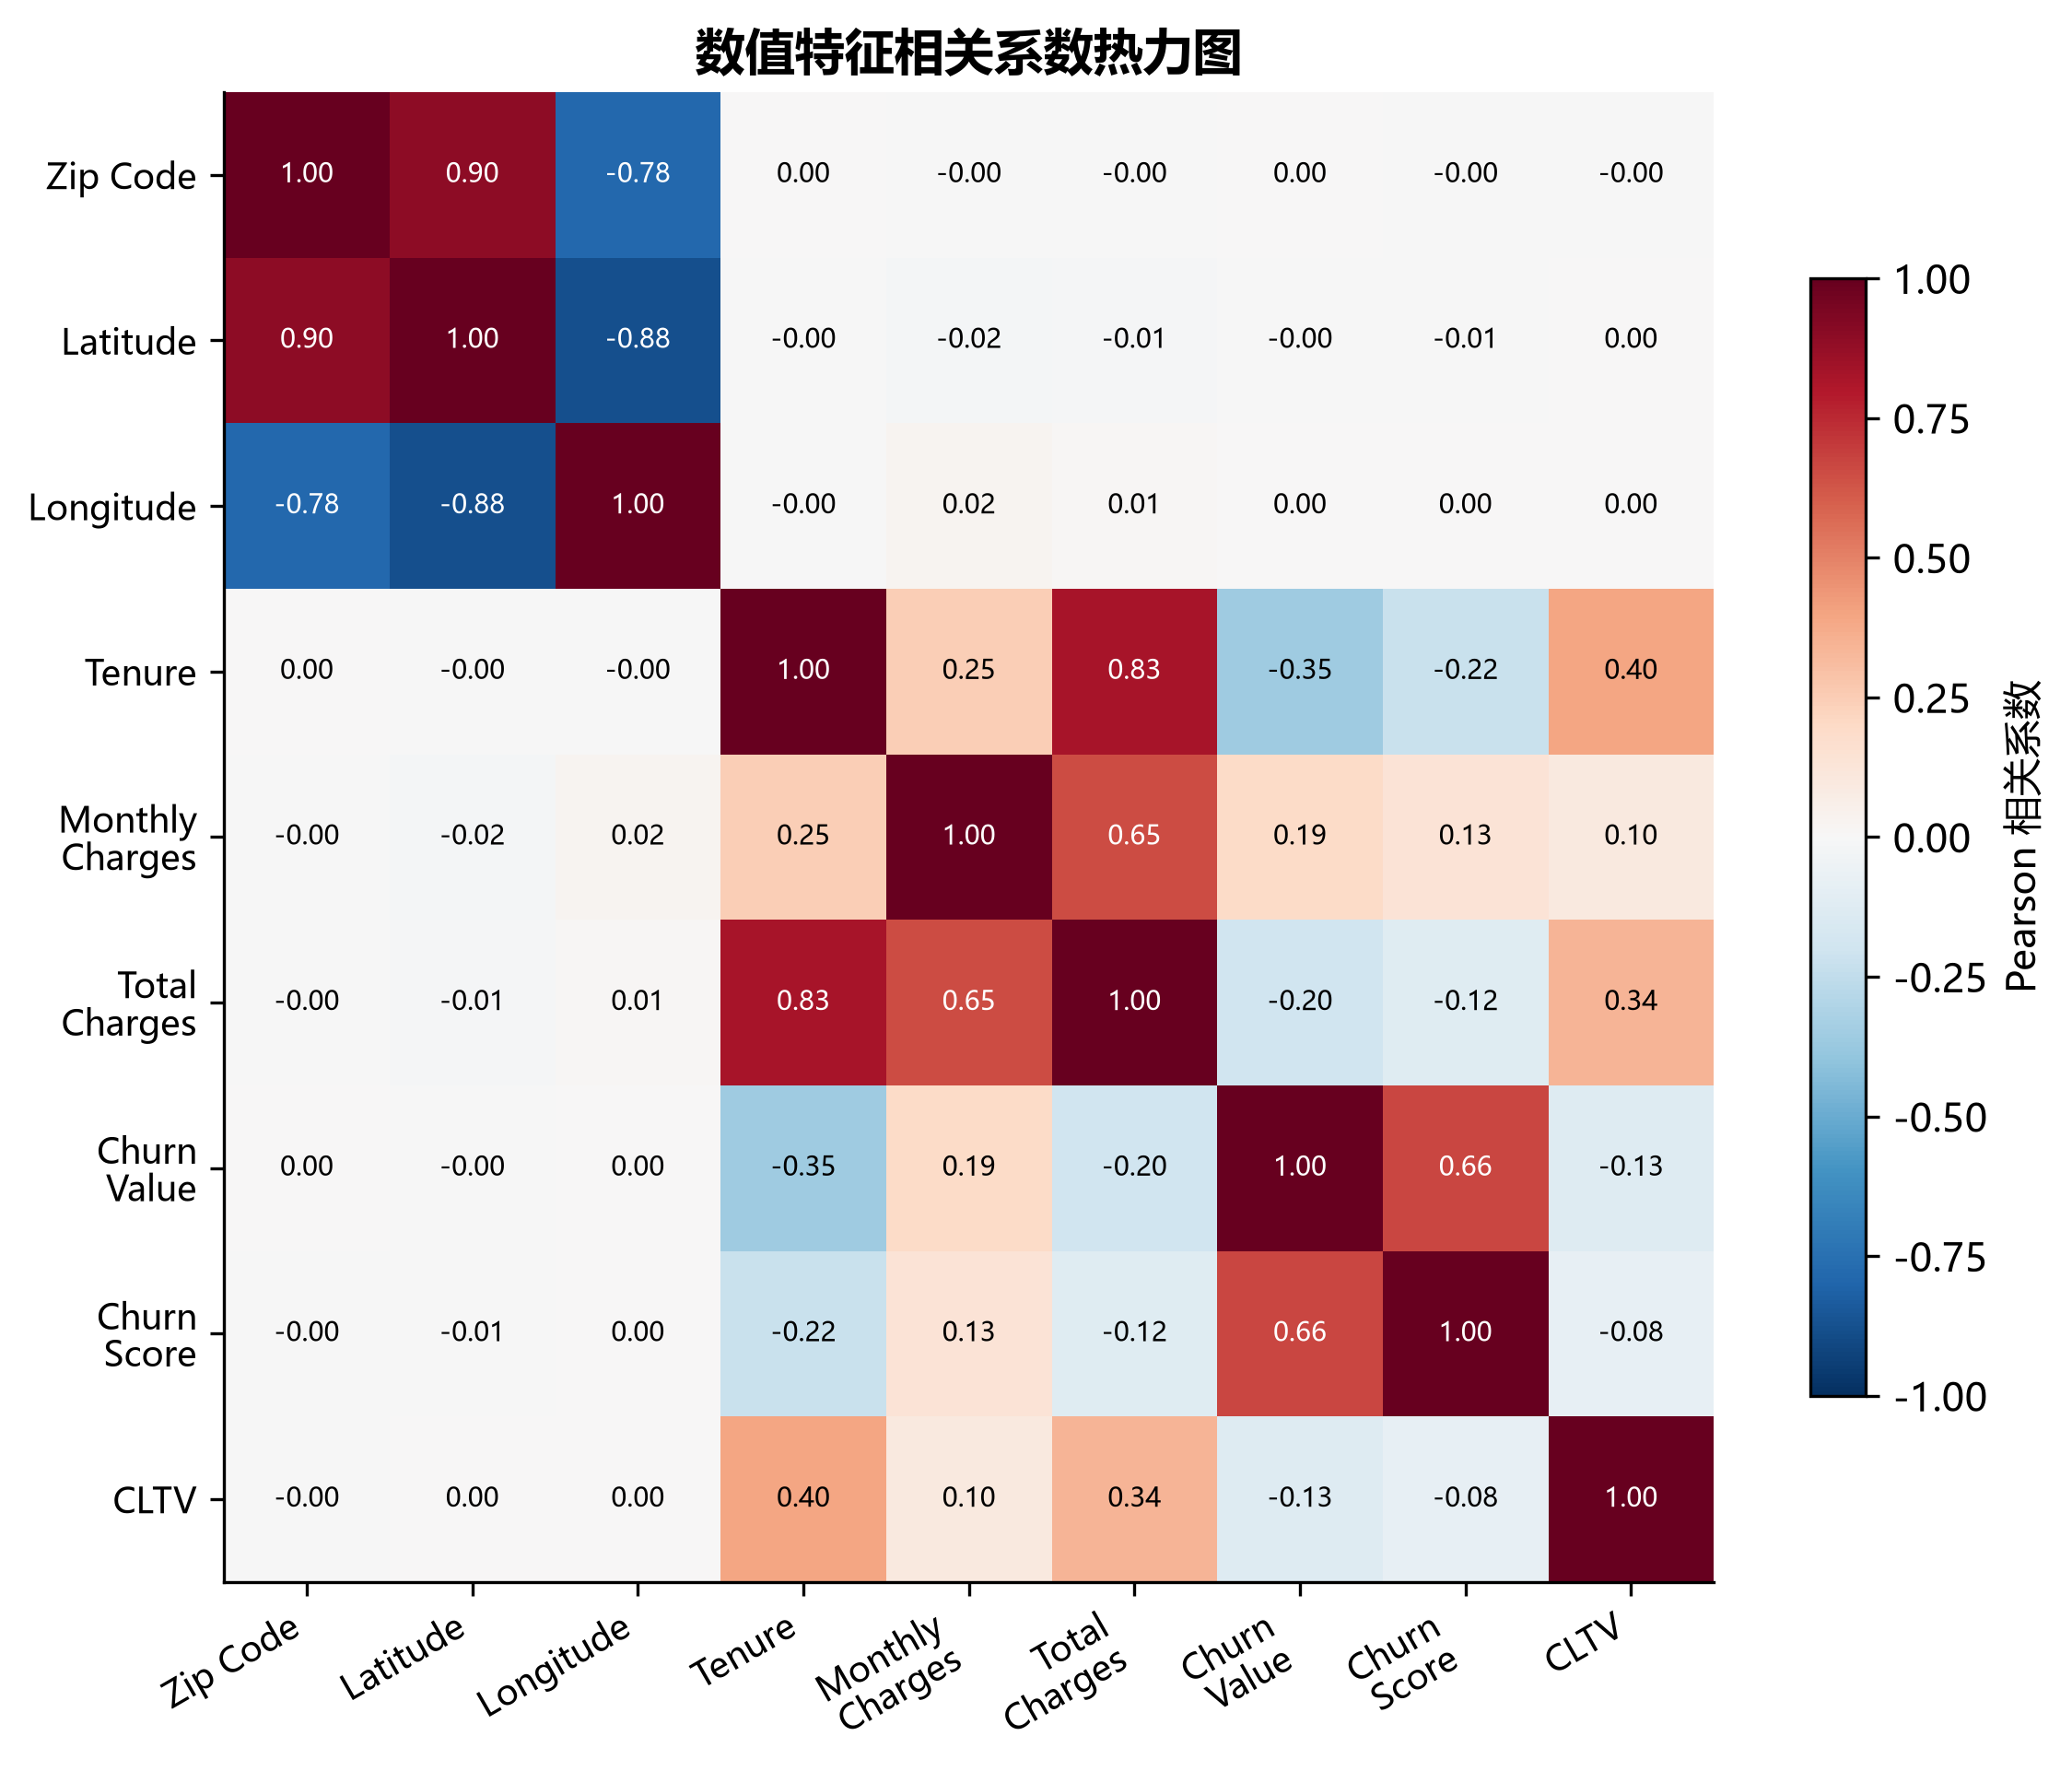
\includegraphics[width=0.75\textwidth]{figures/相关性热力图.png}
    \caption{相关性热力图}
    \label{fig:corr}
\end{figure}

通过热力图可以直观看出各特征与客户流失的相关程度。本文对相关系数的分析，
得到以下发现：

\textbf{在网时长：}与流失的相关系数为 $-0.352$，在所有数值特征中绝对值最大，
呈中等程度的负相关——在网时间越长，流失可能性越低，这与前文分析中
"新客户是高危群体"的结论相一致。

\textbf{月消费金额：}与流失的相关系数为 $+0.193$，呈弱正相关——月消费越高的客户
对服务性价比的要求也越高，流失意愿更强，这与分类特征分析中光纤客户
流失率较高的发现互为印证。

\textbf{总消费金额与CLTV：}与流失的相关系数分别为 $-0.198$ 和 $-0.127$，
均为弱负相关，方向符合预期。但值得注意的是，在网时长与总消费之间存在较强的
正相关（$r = 0.83$），这是因为在网时间越长累计消费自然越高，
说明两变量存在多重共线性，后续建模中可考虑择一保留。

\textbf{地理特征：}经度、纬度、邮编三个特征与流失的相关系数绝对值均小于 $0.01$，
不具备线性预测价值，说明地理位置与客户的流失决策之间不存在明显的关联关系。

\subsubsection{初步结论}

综合上述探索性分析，可从以下维度刻画流失客户的典型特征：
在合同层面，流失客户以月付合同为主，其流失率超过 40\%，
远高于年付和两年合同客户；在在网时长层面，流失客户高度集中在
在网 0-10 个月的新客户群体，在网时长是与流失相关性最强的数值特征
（$r = -0.352$）；在消费层面，流失客户的月消费金额偏高，
高消费群体对服务性价比更为敏感，流失意愿更强；
在家庭层面，无配偶、无家属的独身客户流失率高于有家庭绑定的客户，
前者离网成本更低。

上述发现为下一节分类模型的建立提供了明确的方向——
模型应重点纳入合同类型、在网时长、月消费金额等具有强区分能力的特征变量。
